% Performance teaser plot for mwpm.
%
% Build with:  latexmk -pdf perf.tex
% (uses pdflatex; libertine + newtxmath give Linux Libertine / Biolinum.)

\documentclass[tikz,border=10pt]{standalone}

\usepackage[T1]{fontenc}
\usepackage[mono=false]{libertine}     % Linux Libertine (serif) + Biolinum (sans)
\usepackage[libertine]{newtxmath}      % matching math italics
\usepackage{pgfplots}
\pgfplotsset{compat=1.18}

% A muted, print-friendly palette.
\definecolor{cBF}{HTML}{C0392B}        % brute force      -- alizarin red
\definecolor{cDP}{HTML}{B9770E}        % interval DP      -- dark amber
\definecolor{cSMAWK}{HTML}{1A5276}     % Marcotte & Suri (SMAWK) -- deep navy
\definecolor{cScan}{HTML}{5DADE2}      % Marcotte & Suri (scan)  -- soft blue

\begin{document}
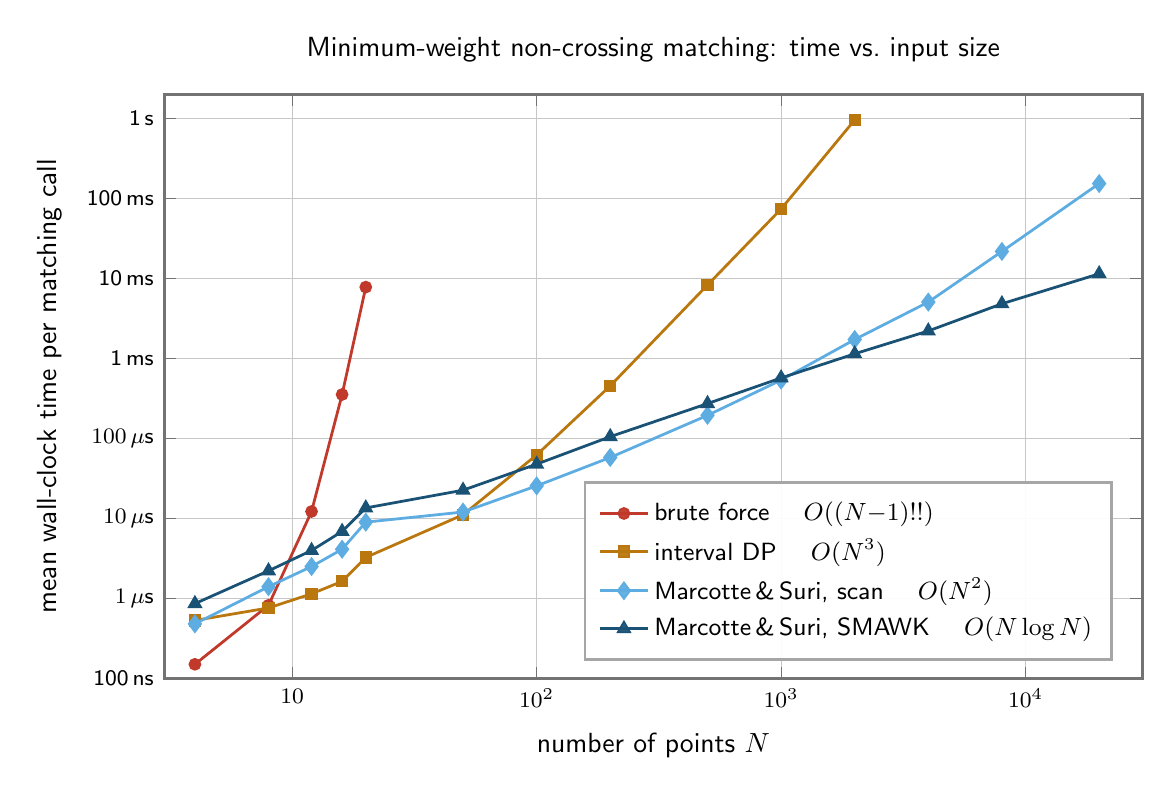
\begin{tikzpicture}

\begin{axis}[
    width=14cm, height=9cm,
    xmode=log, ymode=log,
    log basis x={10}, log basis y={10},
    xmin=3, xmax=30000,
    ymin=1e-7, ymax=2,
    xtick={1,10,100,1000,10000},
    xticklabels={$1$,$10$,$10^2$,$10^3$,$10^4$},
    minor x tick num=8,
    ytick={1e-7,1e-6,1e-5,1e-4,1e-3,1e-2,1e-1,1e0},
    yticklabels={
      100\,ns,
      $1\,\mu$s,
      $10\,\mu$s,
      $100\,\mu$s,
      1\,ms,
      10\,ms,
      100\,ms,
      1\,s
    },
    minor y tick num=8,
    xlabel={number of points $N$},
    ylabel={mean wall-clock time per matching call},
    title={\textsf{Minimum-weight non-crossing matching: time vs.\ input size}},
    title style={yshift=2pt, font=\sffamily},
    xlabel style={yshift=-2pt, font=\sffamily},
    ylabel style={yshift=2pt, font=\sffamily},
    tick label style={font=\sffamily\footnotesize},
    grid=both,
    major grid style={line width=.35pt, draw=black!22},
    minor grid style={line width=.15pt, draw=black!10},
    axis line style={draw=black!55},
    tick style={draw=black!55},
    legend pos=south east,
    legend cell align=left,
    legend style={
      font=\sffamily\small,
      draw=black!35,
      fill=white,
      fill opacity=0.94,
      text opacity=1,
      inner sep=5pt,
      row sep=1pt,
    },
    line width=1.0pt,
    mark options={solid, line width=0.6pt},
    clip mode=individual,
]

% Brute force, capped at N=20 (factorial blow-up after that).
\addplot[color=cBF, mark=*, mark size=2.0pt] coordinates {
    (4,    1.5e-7)
    (8,    8.2e-7)
    (12,   1.22e-5)
    (16,   3.53e-4)
    (20,   7.77e-3)
};
\addlegendentry{brute force \quad $O((N{-}1)!!)$}

% Interval DP, skipped above N=2000 in this sweep.
\addplot[color=cDP, mark=square*, mark size=1.9pt] coordinates {
    (4,    5.3e-7)
    (8,    7.6e-7)
    (12,   1.14e-6)
    (16,   1.63e-6)
    (20,   3.25e-6)
    (50,   1.11e-5)
    (100,  6.21e-5)
    (200,  4.53e-4)
    (500,  8.26e-3)
    (1000, 7.37e-2)
    (2000, 9.54e-1)
};
\addlegendentry{interval DP \quad $O(N^{3})$}

% Marcotte & Suri with simple O(N^2) scan conquer.
\addplot[color=cScan, mark=diamond*, mark size=3.0pt] coordinates {
    (4,     4.8e-7)
    (8,     1.40e-6)
    (12,    2.50e-6)
    (16,    4.11e-6)
    (20,    8.97e-6)
    (50,    1.20e-5)
    (100,   2.55e-5)
    (200,   5.77e-5)
    (500,   1.94e-4)
    (1000,  5.35e-4)
    (2000,  1.72e-3)
    (4000,  5.05e-3)
    (8000,  2.17e-2)
    (20000, 1.53e-1)
};
\addlegendentry{Marcotte\,\&\,Suri, scan \quad $O(N^{2})$}

% Marcotte & Suri with SMAWK conquer.
\addplot[color=cSMAWK, mark=triangle*, mark size=2.6pt] coordinates {
    (4,     8.6e-7)
    (8,     2.21e-6)
    (12,    3.97e-6)
    (16,    6.87e-6)
    (20,    1.35e-5)
    (50,    2.25e-5)
    (100,   4.76e-5)
    (200,   1.05e-4)
    (500,   2.72e-4)
    (1000,  5.69e-4)
    (2000,  1.14e-3)
    (4000,  2.20e-3)
    (8000,  4.81e-3)
    (20000, 1.14e-2)
};
\addlegendentry{Marcotte\,\&\,Suri, SMAWK \quad $O(N\log N)$}

\end{axis}
\end{tikzpicture}
\end{document}
